\chapter{Figures And Charts}

\begin{figure}[hbtp]
  \centering
  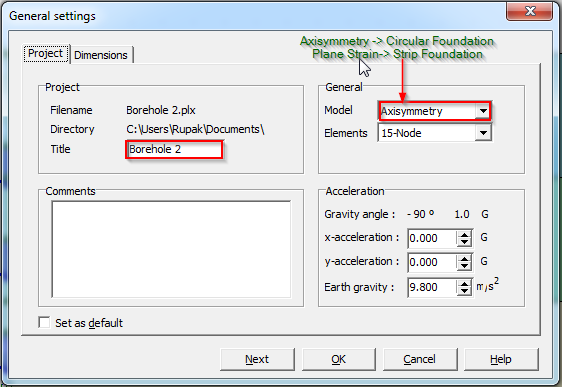
\includegraphics[height=0.33\textheight]{images/plx/a (1).png}
  \caption{Project Options}
  \vfill
  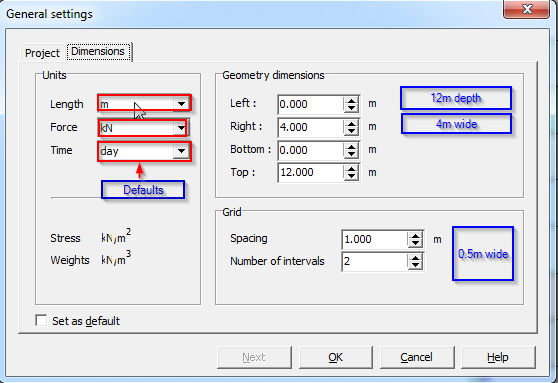
\includegraphics[height=0.33\textheight]{images/plx/a (2).png}
  \caption{Dimension Options}
\end{figure}
\break
\begin{landscape}
\begin{figure}[hbtp]
  \centering
  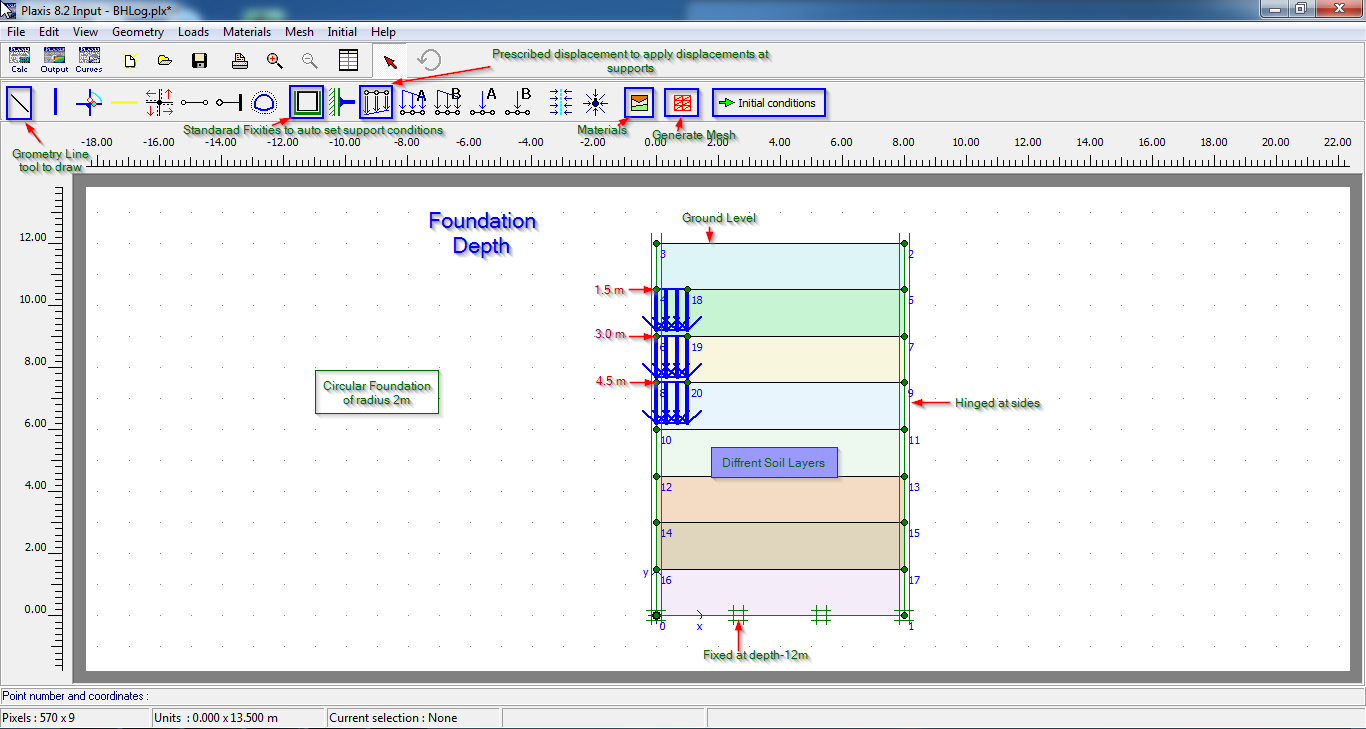
\includegraphics[width=\linewidth, height=\textheight,keepaspectratio]{images/plx/a (4).png}
  \caption{Main drawing page}
\end{figure}
\end{landscape}
\break
\begin{landscape}
\begin{figure}[hbtp]
  \centering
  \hfill
  \begin{minipage}[c]{0.4\linewidth}
  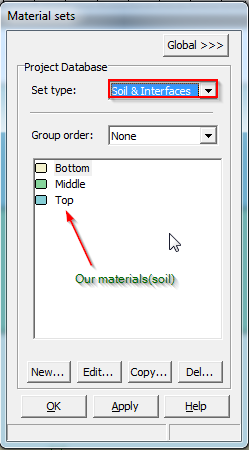
\includegraphics[width=\linewidth, height=\textheight,keepaspectratio]{images/plx/a (3).png}
  \caption{Soil List(Materials)}
  \end{minipage}
  \hfill
  \begin{minipage}[c]{0.4\linewidth}
  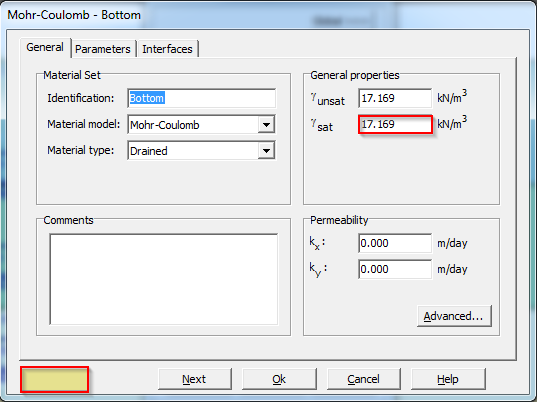
\includegraphics[width=\linewidth, height=0.4\textheight,keepaspectratio]{images/plx/a (6).png}
  \caption{General Soil Parameters}
  \vfill
  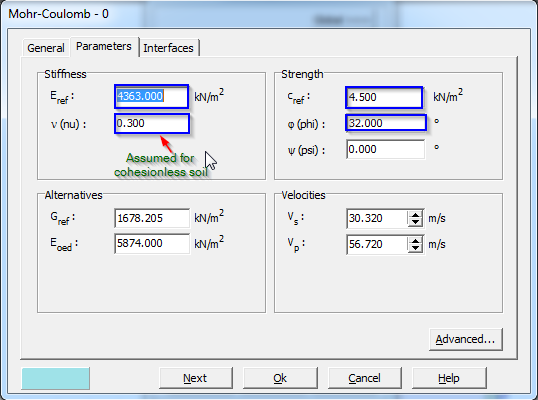
\includegraphics[width=\linewidth, height=0.4\textheight,keepaspectratio]{images/plx/a (7).png}
  \caption{Other Soil Parameters}
  \end{minipage}
  \hfill
\end{figure}
\end{landscape}
\break
\begin{figure}[hbtp]
  \centering
  \vfill
  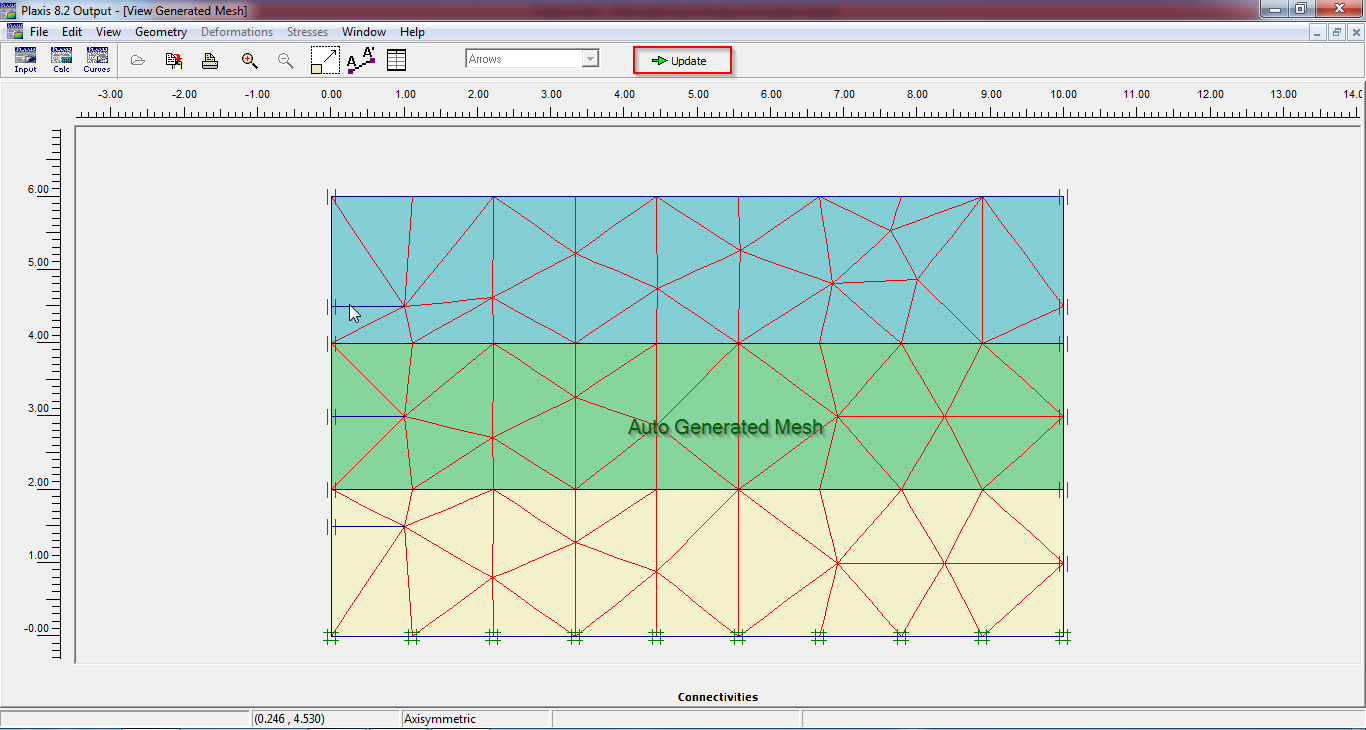
\includegraphics[width=\linewidth, height=0.4\textheight,keepaspectratio]{images/plx/a (5).png}
  \caption{Auto generated mesh}
  \vfill
  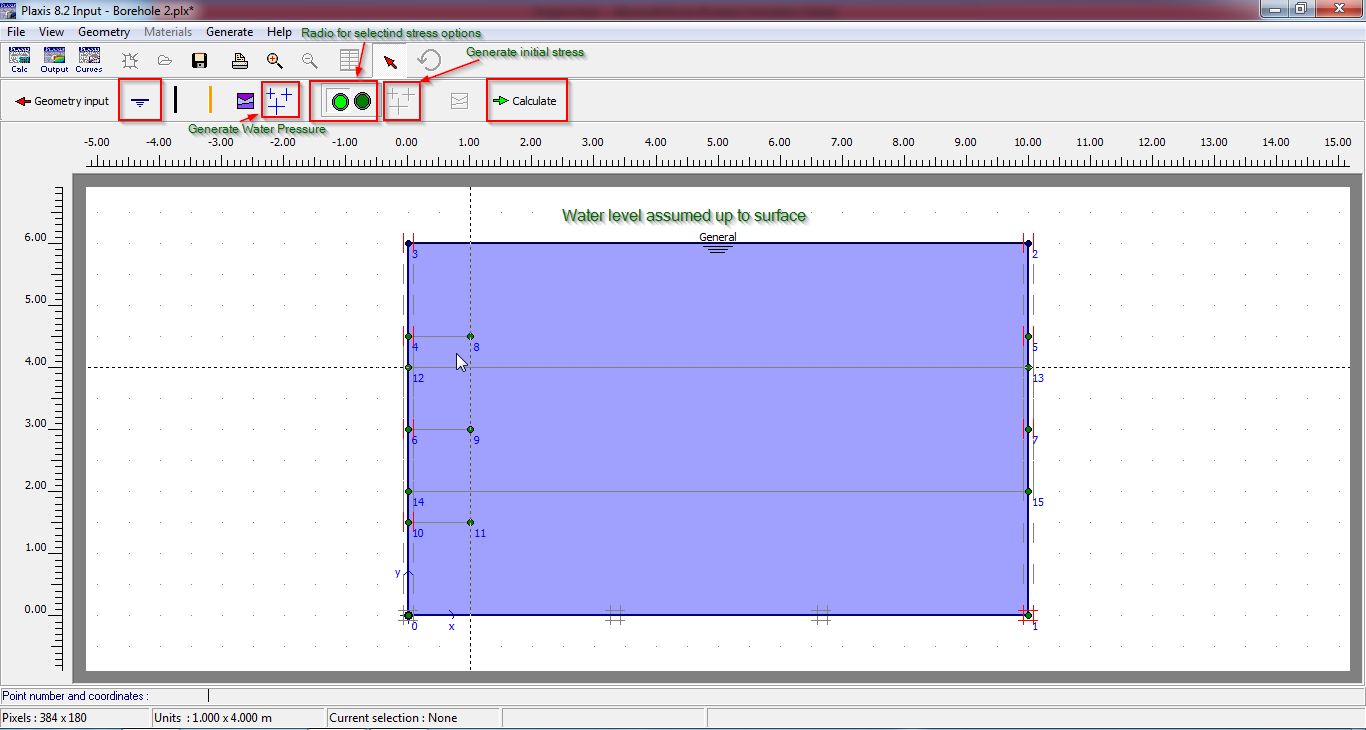
\includegraphics[width=\linewidth, height=0.4\textheight,keepaspectratio]{images/plx/a (8).png}
  \caption{Ground Water Options}
  \vfill
\end{figure}
\break
\begin{landscape}
\begin{figure}[hbtp]
  \centering
  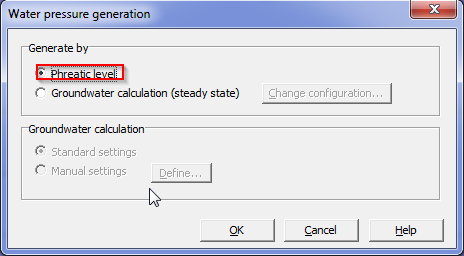
\includegraphics[height=0.25\textheight]{images/plx/a (9).png}
  \caption{Water pressure generation options}
  \vfill
  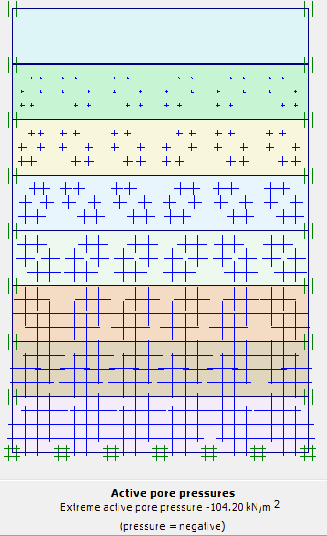
\includegraphics[height=0.65\textheight]{images/plx/a (10).png}
  \caption{Generated pore water pressures}
\end{figure}
\end{landscape}
\break
\begin{landscape}
\begin{figure}[hbtp]
  \centering
  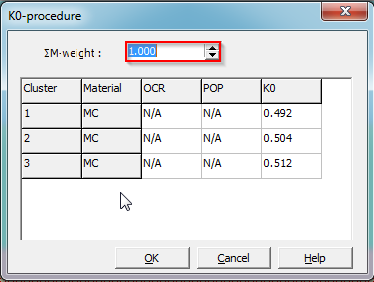
\includegraphics[height=0.25\textheight]{images/plx/a (11).png}
  \caption{Soil pressure generation options}
  \vfill
  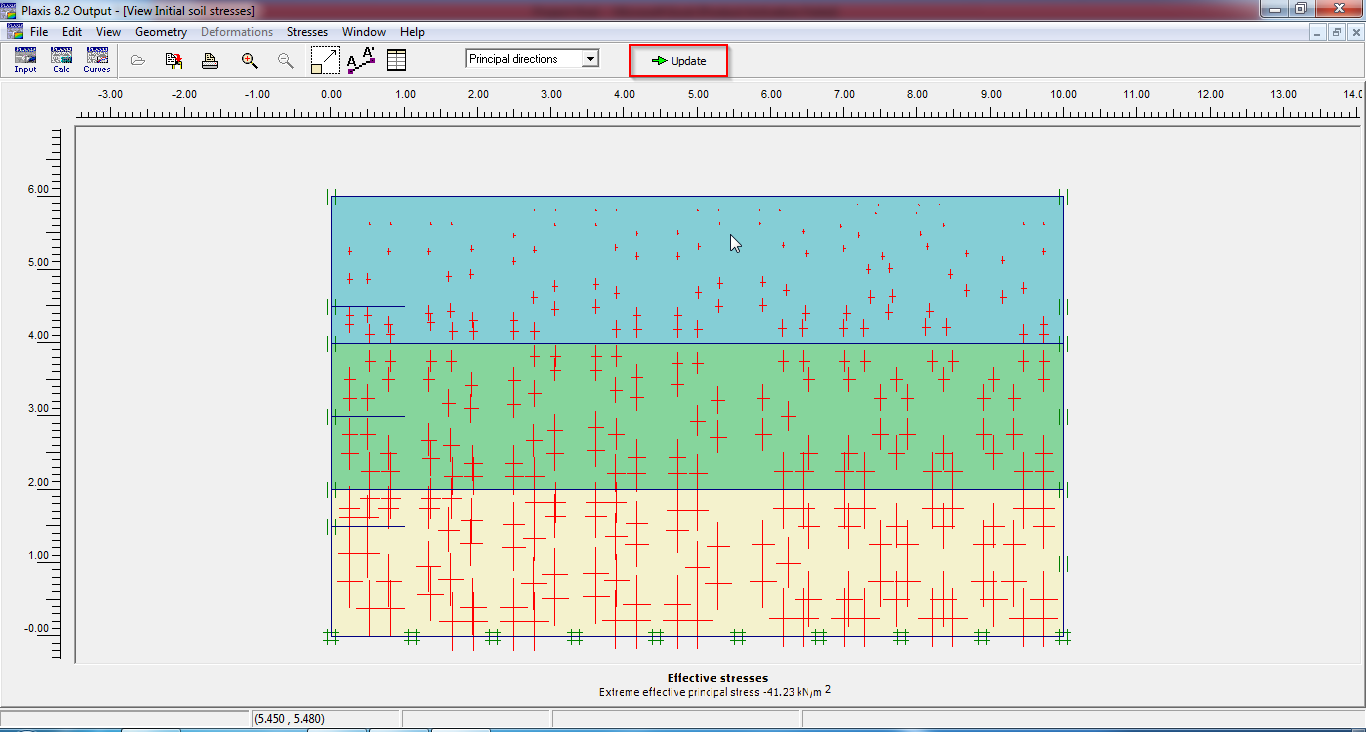
\includegraphics[height=0.65\textheight]{images/plx/a (12).png}
  \caption{Generated soil pressures}
\end{figure}
\end{landscape}
\break
\begin{figure}[hbtp]
  \vfill
  \centering
  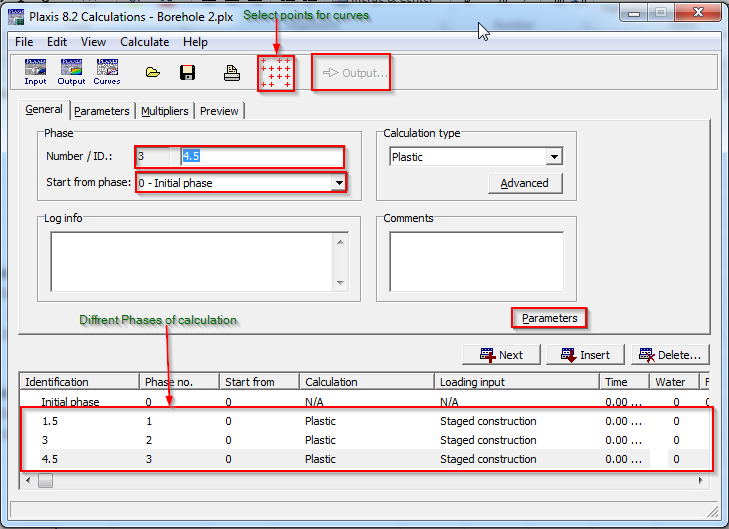
\includegraphics[height=0.4\textheight]{images/plx/a (13).png}
  \caption{Main calculation dialog}
  \vfill
  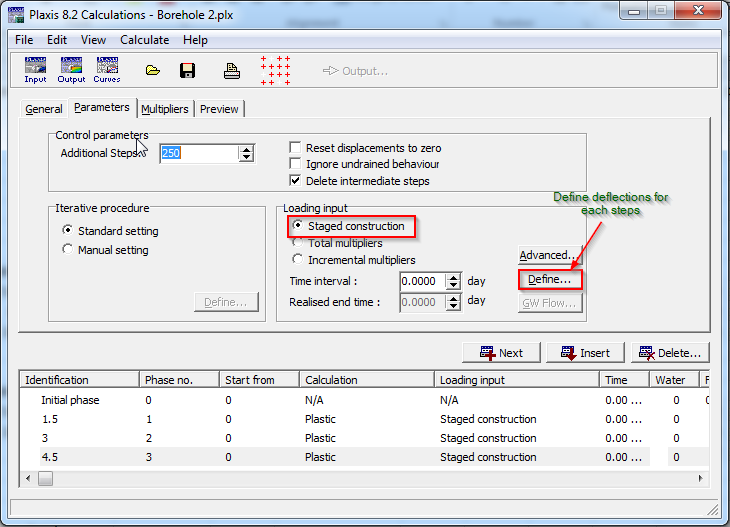
\includegraphics[height=0.4\textheight]{images/plx/a (14).png}
  \caption{Parameters tab}
  \vfill
\end{figure}
\break
\begin{landscape}
\begin{figure}[hbtp]
  \vfill
  \centering
  \begin{minipage}[c]{0.35\linewidth}
    \vfill
    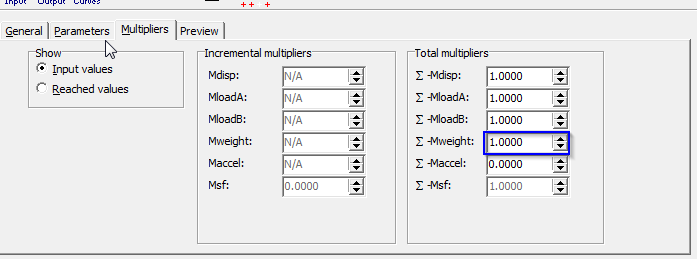
\includegraphics[width=\linewidth, height=0.7\textheight,keepaspectratio]{images/plx/a (15).png}
    \caption{Define Dialog (Select active displacements)}
    \vfill
    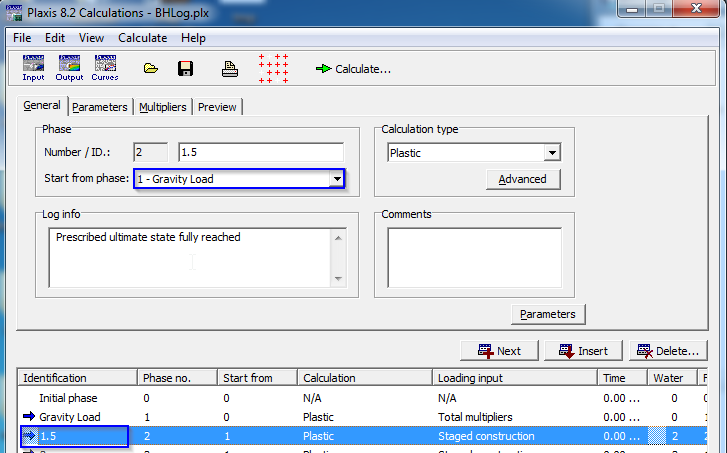
\includegraphics[width=\linewidth, height=0.3\textheight,keepaspectratio]{images/plx/a (16).png}
    \caption{Prescribed displacement dialog}
    \vfill
  \end{minipage}
  \hfill
  \begin{minipage}[c]{0.6\linewidth}
  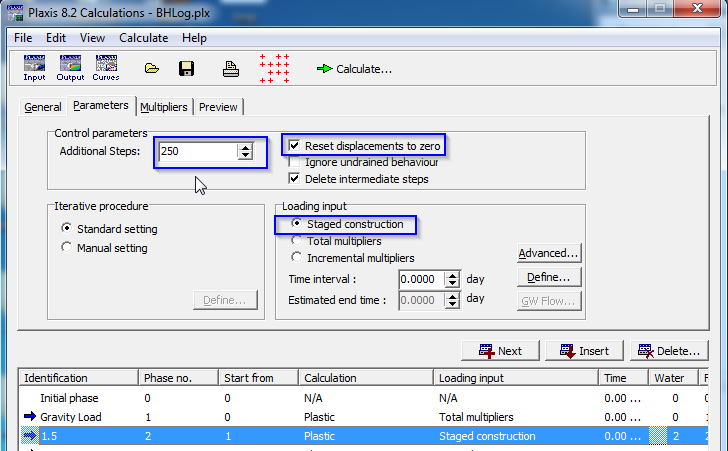
\includegraphics[width=\linewidth, height=\textheight,keepaspectratio]{images/plx/a (17).png}
  \caption{Final Result}
  \end{minipage}
\vfill
\end{figure}
\end{landscape}
\break